\documentclass{article}

% arxiv-standard packages
\usepackage[preprint]{neurips_2024}   % swap to [final] for camera-ready
\usepackage[utf8]{inputenc}
\usepackage[T1]{fontenc}
\usepackage{hyperref}
\usepackage{url}
\usepackage{booktabs}
\usepackage{amsfonts}
\usepackage{amsmath}
\usepackage{amssymb}
\usepackage{nicefrac}
\usepackage{microtype}
\usepackage{xcolor}
\usepackage{graphicx}
\usepackage{algorithm}
\usepackage{algorithmic}
\usepackage{multirow}
\usepackage{tabularx}

\title{Dynamic Attentional Context Scoping:\\
Agent-Triggered Focus Sessions for\\
Isolated Per-Agent Steering in Multi-Agent LLM Orchestration}

\author{%
  Nickson Patel \\
  \texttt{nicksonpatel@gmail.com} \\
  \texttt{nickson@x-algo.net}
}

\begin{document}
\maketitle

%-----------------------------------------------------------------------
\begin{abstract}
Multi-agent LLM orchestration systems suffer from \emph{context pollution}:
when $N$ concurrent agents compete for the orchestrator's context window,
each agent's task state, partial outputs, and pending questions contaminate
the steering interactions of every other agent, degrading decision quality.
We introduce \textbf{Dynamic Attentional Context Scoping (DACS)}, a
mechanism in which the orchestrator operates in two asymmetric modes.
In \textsc{Registry} mode it holds only lightweight per-agent status
summaries ($\leq 200$ tokens each), remaining responsive to all agents
and the user.
When an agent emits a \textsc{SteeringRequest}, the orchestrator enters
\textsc{Focus}$(a_i)$ mode, injecting the full context of agent $a_i$
while compressing all other agents to their registry entries.
Context isolation is agent-triggered, asymmetric, and deterministic:
the context window contains exactly $F(a_i) + R_{-i}$ during steering,
eliminating cross-agent contamination without requiring context
compression or retrieval.
We evaluate DACS across three experimental phases totalling 160 trials:
Phase~1 tests $N \in \{3,5,10\}$ agents (60 trials);
Phase~2 tests agent heterogeneity and adversarial dependency structures
(60 trials);
Phase~3 tests decision density scaling up to $D=15$ steering requests per
agent (40 trials).
Across all 8 scenarios, DACS achieves $90.0$--$98.4\%$ steering accuracy
versus $21.0$--$60.0\%$ for a flat-context baseline ($p < 0.0001$
throughout).
Wrong-agent contamination is $0.0$--$14.0\%$ under DACS versus
$28$--$57\%$ under the baseline.
The accuracy advantage grows with agent count ($N$) and with
decision density ($D$): at $N=3, D=15$, the gap reaches $+54.2$ pp
versus $+36.7$ pp at $N=3, D\approx3$.
DACS context size grows sub-linearly with both $N$ and $D$ while the
baseline grows near-linearly, yielding context efficiency ratios of
up to $3.53\times$.
The keyword matching metric is validated by independent LLM-as-judge
evaluations across all three phases (Phase~2: $\kappa=0.956$;
Phase~3 s8: $\kappa=0.886$; Phase~3 s7: $\kappa=0.933$;
mean $\kappa=0.909$).
All code and data are released at
\href{https://github.com/nicksonpatel/dacs-agent-focus-mode}{\texttt{github.com/nicksonpatel/dacs-agent-focus-mode}}.
\end{abstract}

%-----------------------------------------------------------------------
\section{Introduction}
\label{sec:intro}

The deployment of LLMs as orchestrators managing multiple parallel agents
has become a practical reality: systems such as Claude Code Agent
Teams~\citep{anthropic2025code}, OpenCode~\citep{opencode2025}, and
production multi-agent platforms~\citep{agentorchestra2025} demonstrate
that complex long-horizon tasks can be decomposed across concurrent
specialized agents.
The common architectural choice is a single LLM instance (the
\emph{orchestrator}) that coordinates all agents, handles user
interaction, and steers individual agents when they reach decision points.

\paragraph{The context pollution problem.}
This architecture introduces a fundamental scaling problem.
When $N$ agents run concurrently, each maintains its own task context:
partial outputs, domain-specific state, pending decisions.
In a flat-context orchestrator, all of these threads compete for space in
a single context window.
When agent $a_i$ requests steering—``should I use BFS or DFS for this
graph traversal?''—the orchestrator's context simultaneously holds $a_j$'s
transformer attention survey, $a_k$'s CSV encoding problem, and so on.
We call this \emph{context pollution}: the systematic contamination of
one agent's steering interaction by irrelevant context from other agents.

The consequences are measurable and severe.
Prior work has documented context pollution in single-agent settings
under tool overload~\citep{adaptorch2025,codedelegator2025}, under
retrieval bloat~\citep{sidequest2025}, and under long conversation
histories~\citep{afm2024,ace2026}.
Our experiments show that in the multi-agent setting, a flat-context
orchestrator's steering accuracy collapses from 60\% at $N=3$ to 21\% at
$N=10$ (Phase~1), and further degrades as agents become more diverse
(Phase~2) or accumulate longer decision histories (Phase~3).

\paragraph{The DACS mechanism.}
We propose \textbf{Dynamic Attentional Context Scoping (DACS)}, which
solves context pollution through \emph{agent-triggered asymmetric context
isolation}.
DACS introduces two orchestrator modes:

\begin{itemize}
  \item \textbf{\textsc{Registry} mode.} The orchestrator holds only the
  registry $R = \{r_1, \ldots, r_N\}$—one compact status summary per
  agent ($\leq 200$ tokens each).
  It monitors all agents, responds to the user, and queues incoming
  steering requests.

  \item \textbf{\textsc{Focus}$(a_i)$ mode.} When agent $a_i$ emits a
  \textsc{SteeringRequest}, the orchestrator transitions to hold $F(a_i)$
  (the full context of $a_i$: task description, prior steering exchanges,
  current partial output) plus a compressed version of $R_{-i}$
  (registry summaries for all agents except $a_i$).
  The context window contains exactly what is needed to steer $a_i$,
  and nothing from any other agent's task thread.
\end{itemize}

The key properties of DACS that distinguish it from prior context
management approaches are:
\begin{enumerate}
  \item \textbf{Agent-triggered.} Context isolation fires when an agent
  needs it, not on every turn or at task-decomposition time.
  \item \textbf{Asymmetric.} The steered agent gets full fidelity;
  all others get compressed summaries.
  \item \textbf{Exact, not approximate.} No scoring function, no fidelity
  tiering~\citep{afm2024,lemon2025}, no probabilistic compression—the
  context is deterministically constructed as $F(a_i) + R_{-i}$.
  \item \textbf{Sub-linear in $N$ and $D$.} Focus context size is
  independent of the number of other agents; only the compressed registry
  grows with $N$ (by $\approx 25$ tokens per additional agent in our
  experiments). Accuracy is also stable as decision density $D$ increases.
\end{enumerate}

\paragraph{Contributions.}
\begin{enumerate}
  \item We formally define the DACS mechanism: the \textsc{Registry}/
  \textsc{Focus} state machine, the \textsc{SteeringRequest} protocol,
  and the context builder invariants (\S\ref{sec:mechanism}).
  \item We implement a minimal, fully observable orchestration harness
  ($\sim$300 lines) where every token entering each LLM call is logged,
  enabling strict experimental control (\S\ref{sec:experiments}).
  \item We show large, statistically significant accuracy gains across
  Phase~1 ($N$ scaling), Phase~2 (agent diversity and adversarial
  dependencies), and Phase~3 (decision density scaling), together
  answering four distinct research questions (\S\ref{sec:results}).
  \item We independently validate the keyword matching metric with
  LLM-as-judge evaluations across all three phases (Phase~2: $\kappa=0.956$;
  Phase~3: mean $\kappa=0.909$), confirming that reported advantage sizes
  are robust (\S\ref{sec:results}).
  \item We identify sub-linear context scaling as the mechanism's key
  theoretical property, explain its source, and discuss conditions under
  which it holds (\S\ref{sec:discussion}).
\end{enumerate}

%-----------------------------------------------------------------------
\section{Related Work}
\label{sec:related}

Context management for LLM agents has been studied at three levels of
granularity: single-agent memory across turns, single-agent tool/retrieval
bloat, and multi-agent orchestration.
DACS addresses a problem at the third level that existing work at the
first two levels does not reach.

\paragraph{Single-turn context compression.}
AFM~\citep{afm2024} assigns per-message fidelity tiers
(Full/Compressed/Placeholder) based on a composite recency-relevance score
and packs messages greedily under a token budget.
It achieves 83.3\% constraint-recall on its benchmark, validating that
structured fidelity management outperforms naive truncation.
ACE~\citep{ace2026} treats the agent's context as an evolving playbook
of itemized bullets with utility counters, using incremental delta updates
to avoid context collapse (they observe a 18{,}282-token context collapsing
to 122 tokens under iterative rewriting, dropping accuracy below the
no-adaptation baseline).
Both AFM and ACE operate within a single agent's context history.
Neither addresses $N$ concurrent agents competing for an orchestrator
context window, and neither models wrong-agent contamination as a failure
mode.

\paragraph{Retrieval and cache bloat.}
SideQuest~\citep{sidequest2025} frames KV cache compression as an
auxiliary task solved by the LRM itself, achieving 65\% peak token
reduction on single-agent deep research tasks.
Lemon Agent~\citep{lemon2025} applies three-tier progressive compression
(full → compressed → summary) to a shared orchestrator context over task
time in an orchestrator-worker system.
Both treat context as a resource to compress; neither introduces asymmetric
isolation triggered by an agent's request.

\paragraph{Context pollution in tool-heavy agents.}
Adaptive Orchestration~\citep{adaptorch2025} identifies context pollution
and attention decay as failure modes in monolithic agents loaded with too
many tools, and proposes spawning specialist sub-agents (DMoE) to offload
capability.
CodeDelegator~\citep{codedelegator2025} separates planner and executor
roles via Ephemeral-Persistent State Separation (EPSS): a persistent
Delegator never receives execution traces; each Coder sub-task starts with
a clean context.
Both solve context pollution \emph{architecturally} (at task decomposition
time) for sequential delegation to one sub-agent at a time.
DACS solves it \emph{dynamically at runtime}, during the steering
interaction itself, for $N$ agents running simultaneously.
The distinction matters: CodeDelegator's Delegator has no mechanism for
handling the case where multiple concurrent Coders simultaneously need
steering.

\paragraph{Multi-agent orchestration context management.}
AOI~\citep{aoi2024} introduces a three-layer memory architecture for
multi-agent IT operations, with a central Context Compressor transforming
raw agent outputs into a compressed cache.
Its Observer agent always holds a compressed aggregate of \emph{all}
agent activity simultaneously—there is no per-agent isolation.
Agents execute and report results; they cannot signal the orchestrator
for steering attention, and wrong-agent contamination is not modelled
(AOI's failure mode is information loss from operational data volume).
AgentOrchestra~\citep{agentorchestra2025} achieves SOTA on GAIA (89.04\%)
via hierarchical delegation: a planning agent routes sub-tasks to
domain-specific sub-agents, bounding the planner's context footprint by
converting global coordination into localized routing decisions.
The paper explicitly notes that flat coordination ``tends to accumulate
irrelevant context''—independent validation of the problem DACS solves.
However, hierarchical routing is a structural (pre-execution) partial
solution: it reduces \emph{how much} context enters the orchestrator, but
agents still request the orchestrator's attention concurrently at runtime,
and the orchestrator has one flat context window for those interactions.
DACS and AgentOrchestra are complementary: AgentOrchestra reduces the
initial context volume; DACS controls what the orchestrator holds at the
moment of each steering decision.
AdaptOrch~\citep{adaptorch2025b} formalizes topology selection as the
dominant performance variable as frontier LLMs converge, showing
$+6.9$--$9.8$pp gains on SWE-bench/GPQA/HotpotQA from topology-aware
routing.
AdaptOrch makes one topology decision per task; DACS makes repeated
context-switch decisions throughout execution.

\paragraph{Summary.}
No prior work implements agent-triggered asymmetric \textsc{Registry}/
\textsc{Focus} mode switching for per-agent context isolation in
concurrent multi-agent orchestration.
Table~\ref{tab:related} summarises the key distinctions.

\begin{table}[t]
\caption{Comparison of context management mechanisms.}
\label{tab:related}
\centering
\small
\begin{tabular}{lcccc}
\toprule
\textbf{System} & \textbf{$N$ concurrent} & \textbf{Asym.\ mode switch} & \textbf{Agent-triggered} & \textbf{Contamination metric} \\
\midrule
AFM              & \texttimes & \texttimes & \texttimes & \texttimes \\
ACE              & \texttimes & \texttimes & \texttimes & \texttimes \\
AOI              & \checkmark & \texttimes & \texttimes & \texttimes \\
AgentOrchestra   & \checkmark & \texttimes & \texttimes & \texttimes \\
AdaptOrch        & \checkmark & \texttimes & \texttimes & \texttimes \\
CodeDelegator    & \texttimes & \texttimes & \texttimes & \texttimes \\
Adaptive Orch.   & \texttimes & \texttimes & \texttimes & \texttimes \\
Lemon Agent      & \checkmark & \texttimes & \texttimes & \texttimes \\
\midrule
\textbf{DACS (ours)} & \checkmark & \checkmark & \checkmark & \checkmark \\
\bottomrule
\end{tabular}
\end{table}

%-----------------------------------------------------------------------
\section{Dynamic Attentional Context Scoping (DACS)}
\label{sec:mechanism}

\subsection{Entities and Notation}
\label{sec:notation}

Let $O$ denote the orchestrator LLM, $A = \{a_1, \ldots, a_N\}$ the set
of $N$ concurrently running agents, and $T$ the context window token
budget.
Each agent $a_i$ has an associated \emph{focus context}
$F(a_i)$—the full set of information the orchestrator needs to steer
$a_i$: task description, previous steering exchanges between $O$ and
$a_i$, and $a_i$'s current partial output summary.

The \emph{registry} $R = \{r_1, \ldots, r_N\}$ is a set of compact status
snapshots, one per agent.
Each entry $r_i$ contains:

\begin{center}
\begin{tabular}{ll}
\texttt{agent\_id} & identifier \\
\texttt{task} & task description ($\leq 50$ tokens) \\
\texttt{status} & \textsc{Running} $|$ \textsc{Blocked} $|$ \textsc{Waiting} $|$ \textsc{Complete} \\
\texttt{last\_output\_summary} & $\leq 100$ tokens \\
\texttt{urgency} & \textsc{Low} $|$ \textsc{Medium} $|$ \textsc{High} \\
\end{tabular}
\end{center}

Target budget per entry: $\leq 200$ tokens.
Full registry size for $N=10$: $\leq 2{,}000$ tokens, leaving ample space for $F(a_i)$.

\subsection{Orchestrator State Machine}
\label{sec:fsm}

The orchestrator operates as an explicit finite-state machine with three states:

\begin{description}
  \item[\textsc{Registry}.] $O$ holds $R$ only.
  It monitors all agents, responds to user messages, and processes
  incoming \textsc{SteeringRequest}s from the queue.

  \item[\textsc{Focus}$(a_i)$.] $O$ holds $F(a_i)$ and a compressed view
  of $R_{-i}$ (all registry entries except $a_i$'s, since $a_i$'s full
  context is already in $F(a_i)$).
  $O$ steers $a_i$ and cannot accept new steering requests until the
  focus session ends.

  \item[\textsc{UserInteract}.] $O$ responds to a user message using $R$
  only (same as \textsc{Registry} mode, but explicitly user-facing).
  Queued steering requests are not processed until this state exits.
\end{description}

\noindent\textbf{Transitions:}
\begin{align}
  \textsc{Registry} &\;\to\; \textsc{Focus}(a_i): \quad
    a_i \text{ emits } \textsc{SteeringRequest}(\text{urgency} = \text{any}) \label{eq:t1}\\
  \textsc{Focus}(a_i) &\;\to\; \textsc{Registry}: \quad
    \textsc{SteeringComplete} \text{ or } \textsc{SteeringAbandoned} \label{eq:t2}\\
  \textsc{Focus}(a_i) &\;\to\; \textsc{Focus}(a_j): \quad
    a_j \text{ emits } \textsc{SteeringRequest}(\text{urgency} = \textsc{High}), \; a_j \neq a_i \label{eq:t3}\\
  \textsc{Registry} &\;\to\; \textsc{UserInteract}: \quad
    \text{user message received} \label{eq:t4}
\end{align}

Transition~\eqref{eq:t3} (the \emph{interrupt} protocol) allows a
high-urgency agent to preempt an active focus session.
On interrupt, the current partial steering state for $a_i$ is saved and
a new focus context for $a_j$ is built.
After $a_j$ is steered, the orchestrator returns to $\textsc{Registry}$
and resumes $a_i$'s interrupted session if it is still pending.

\subsection{The SteeringRequest Protocol}
\label{sec:protocol}

When agent $a_i$ reaches a decision point it cannot resolve autonomously,
it emits:

\begin{verbatim}
SteeringRequest {
  agent_id:   str
  context:    str   -- relevant context excerpt
  question:   str   -- specific decision needed
  blocking:   bool  -- is a_i halted?
  urgency:    LOW | MEDIUM | HIGH
}
\end{verbatim}

\textsc{High} urgency can interrupt an active focus session
(transition~\eqref{eq:t3}).
\textsc{Medium} requests queue; the agent continues on a default path.
\textsc{Low} requests are batched.

\subsection{Context Builder}
\label{sec:context_builder}

The context builder constructs the orchestrator's prompt before each LLM
call.
It enforces a hard token budget $T$ deterministically (token count is
checked and enforced before every call; the LLM provider is never relied
upon for truncation).

\begin{description}
  \item[\texttt{build\_focus\_context}$(a_i)$.]
  Returns $F(a_i) \,\|\, \texttt{compress}(R_{-i})$.
  If $|F(a_i)| + |R_{-i}| > T$, registry entries for lower-urgency
  agents are progressively truncated until the budget is met.
  $a_i$'s focus context $F(a_i)$ is never truncated.

  \item[\texttt{build\_registry\_context}$()$.]
  Returns $R$ in full.
  Used during \textsc{Registry} and \textsc{UserInteract} modes.
\end{description}

\noindent\textbf{Invariants enforced by the context builder:}
\begin{enumerate}
  \item $O$ is never simultaneously in \textsc{Focus} mode for more than
  one agent. \label{inv:1}
  \item User messages are never dropped; they are queued during
  \textsc{Focus} and processed on the next \textsc{Registry} entry.
  \item $R$ is always current within the last agent heartbeat (agents push
  a compact status update after each step). \label{inv:3}
  \item $|C| \leq T$ holds before every LLM call without exception. \label{inv:4}
\end{enumerate}

\subsection{Complexity Analysis}
\label{sec:complexity}

Let $|F|$ denote the average focus context size (task-dependent, independent
of $N$) and $|r|$ the average registry entry size ($\leq 200$ tokens).

\paragraph{\textsc{Registry} mode context size.}
$|C_{\text{reg}}| = N \cdot |r|$, growing linearly in $N$.
However, this mode is lightweight—the orchestrator makes no costly
steering decisions here, only monitoring and routing.

\paragraph{\textsc{Focus}$(a_i)$ mode context size.}
$|C_{\text{focus}}| = |F| + (N-1) \cdot |r|$.
The focus context $|F|$ is independent of $N$.
Only the compressed registry of $N-1$ agents adds $O(N)$ tokens.
For large $|F|$ and small $|r|$ (our target design point), this is
approximately $|F| + O(N \cdot |r|)$ where $|r| \ll |F|$.

In Phase~1 experiments, $|F| \approx 450$--$550$ tokens per agent and
$|r| \approx 25$ tokens, giving $|C_{\text{focus}}| \approx 500 + 25N$,
empirically confirmed: 561 tokens at $N=3$, 633 at $N=5$, 816 at $N=10$
($+25.5$ tokens/agent, $R^2 > 0.99$).

In Phase~3 (high decision density, $D=15$), $|F|$ grows with the
accumulated steering history, yielding $|C_{\text{focus}}| \approx 2{,}755$
tokens—higher than Phase~1 in absolute terms, but isolated to exactly
$a_i$'s history.
The flat baseline accumulates \emph{all} agents' histories simultaneously,
reaching 6{,}573 tokens (2.39$\times$ ratio).

\paragraph{Efficiency ratio.}
$\rho(N) = |C_{\text{flat}}| / |C_{\text{focus}}| \approx N|F| / (|F| +
N|r|)$.
As $N \to \infty$, $\rho \to |F| / |r| \approx 20$--$22\times$ at our
design point.
Empirically, $\rho$ grows from 2.12$\times$ ($N=3$) to 3.53$\times$
($N=10$) in Phase~1, and reaches 3.24$\times$ at $N=5, D=8$ in Phase~3.

%-----------------------------------------------------------------------
\section{Experimental Setup}
\label{sec:experiments}

\subsection{Harness Design}
\label{sec:harness}

We implement a minimal Python orchestration harness ($\sim$300 lines
across \texttt{src/}) with full context observability: \emph{every} token
entering each LLM call is logged to a \texttt{.jsonl} trial file.
This is the central experimental variable.
We use no external orchestration framework (LangGraph, CrewAI, etc.)—
their context assembly internals would add uncontrolled noise.

The harness has four components:
\texttt{registry.py} (per-agent state management),
\texttt{protocols.py} (\textsc{SteeringRequest/Response} dataclasses),
\texttt{context\_builder.py} (token-counted context construction),
\texttt{orchestrator.py} (state machine + LLM call dispatch).

\paragraph{LLM backend.}
All experiments use MiniMax-M2.7 via an Anthropic-compatible API endpoint
(token budget 204{,}800).
The same model and endpoint are used for DACS and the baseline, ensuring
no confound from model differences.

\subsection{Conditions}
\label{sec:conditions}

\paragraph{DACS.} Orchestrator operates with full \textsc{Registry}/
\textsc{Focus} mode switching as described in \S\ref{sec:mechanism}.

\paragraph{Baseline (flat context).} All agents' full contexts are
injected simultaneously into every steering call.
The baseline uses the \emph{identical} code path as DACS, with the single
difference that \texttt{build\_focus\_context} is replaced by
\texttt{build\_flat\_context} (concatenates all $F(a_i)$).
No other differences.

\subsection{Task Suite}
\label{sec:tasks}

We design 8 scenarios across three experimental phases,
each with known-correct answers defined per decision point.
Correctness is evaluated by keyword matching: a steering response scores
correct if it contains $\geq 1$ expected ground-truth keyword for agent
$a_i$'s current decision point.
Each agent's correct-answer keywords are domain-specific and orthogonal
to all other agents—cross-agent vocabulary leakage is unambiguous.

\paragraph{Phase~1 — Agent count scaling (RQ1, RQ2).}
Three canonical scenarios vary $N \in \{3, 5, 10\}$ with $D \approx 3$
decisions per agent.

\begin{itemize}
  \item \textbf{s1\_n3} ($N=3$): Code writer (BST), research agent
  (transformer attention survey), data processor (CSV encoding).
  15 steering interactions per trial.

  \item \textbf{s2\_n5} ($N=5$): Above three plus graph algorithm agent
  (BFS/DFS) and RL survey agent.
  15 steering interactions per trial.

  \item \textbf{s3\_n10} ($N=10$): Above five plus federated learning,
  e-commerce churn, LRU cache, LLM alignment, and clinical trial
  pre-processing agents.
  30 steering interactions per trial.
\end{itemize}

\paragraph{Phase~2 — Agent diversity (RQ3).}
Three scenarios probe whether the DACS advantage generalises across
agent heterogeneity structures, including an adversarial case.

\begin{itemize}
  \item \textbf{s4\_n3\_homogeneous} ($N=3, D=4$): Three agents from the
  same domain (algorithm coding: red-black tree, open-addressing hash
  table, directed weighted graph).
  Minimal-contamination case—DACS must help even when domains share
  vocabulary.

  \item \textbf{s5\_n5\_crossfire} ($N=5, D=4$): Five maximally diverse
  domains: lock-free C++ queue, diffusion model survey, genomics VCF
  ETL, C++ memory-leak debugger, clinical trial methodology.
  Guaranteed vocabulary disjointness maximises the contamination signal.

  \item \textbf{s6\_n5\_cascade} ($N=5, D=3$): Five pipeline-dependent
  agents (planner $\to$ retrieval $\to$ ranking $\to$ feature store $\to$
  reviewer in a recommendation system).
  Adversarial for DACS: the flat baseline may benefit from seeing all
  agents' histories simultaneously when outputs depend on each other.
\end{itemize}

\paragraph{Phase~3 — Decision density scaling (RQ4).}
Two scenarios fix low $N$ but raise $D$ substantially to probe whether
DACS advantage compounds with decision history depth.

\begin{itemize}
  \item \textbf{s7\_n5\_dense\_d2} ($N=5, D=8$, 40 total steering
  interactions): Five diverse agents—async web scraper, federated
  learning survey, fraud detection pipeline, flaky-test debugger,
  distributed cache TDD.
  Doubles Phase 1's $D$ at fixed $N=5$.

  \item \textbf{s8\_n3\_dense\_d3} ($N=3, D=15$, 45 total steering
  interactions): Three agents—BERT legal-text classifier training loop,
  clinical trial hypothesis testing, post-quantum cryptography
  whitepaper.
  Quintuples Phase 1's $D$ at fixed $N=3$, the most decision-history-
  intensive scenario tested.
\end{itemize}

\subsection{Metrics}
\label{sec:metrics}

\begin{description}
  \item[\textbf{Steering accuracy.}]
  For each steering interaction, we check whether the orchestrator's
  response contains the expected ground-truth keywords for agent $a_i$.
  Score: fraction of interactions with correct keyword hit, averaged
  across all steering interactions in the trial.

  \item[\textbf{Wrong-agent contamination.}]
  For each steering response targeting $a_i$, we check whether the
  response contains ground-truth keywords for any $a_j$, $j \neq i$.
  Score: fraction of interactions with cross-agent keyword leakage.

  \item[\textbf{Context size at steering.}]
  Token count of the orchestrator's context window at the moment the
  steering LLM call is made.
  Logged directly from the context builder.
\end{description}

\paragraph{Metric validation.}
Keyword matching is validated at two stages via independent LLM-as-judge
evaluations using the same MiniMax-M2.7 model.
In Phase~2 all 400 decisions in \textbf{s5\_n5\_crossfire} were judged:
agreement 98.0\% ($\pm 1.4\%$); Cohen's $\kappa = 0.956$ (near-perfect).
For Phase~3 we ran a stratified judge pass on both dense scenarios:
100 sampled decisions from \textbf{s8\_n3\_dense\_d3} (50 DACS~$+$~50 baseline)
and 200 from \textbf{s7\_n5\_dense\_d2} (100 DACS~$+$~100 baseline).
Agreement: 95.0\% ($\kappa=0.886$) for s8; 97.0\% ($\kappa=0.933$) for s7;
mean $\kappa=0.909$ across both Phase~3 scenarios.
All four judge evaluations ($\kappa \geq 0.886$) establish keyword matching
as a valid proxy for LLM-judged correctness across the full experiment series.

\subsection{Procedure}
\label{sec:procedure}

We run 10 independent trials per condition per scenario (160 total trials:
60 Phase~1, 60 Phase~2, 40 Phase~3).
Each trial uses a fresh agent instantiation with randomised task parameter
order. Phase~3 trials were run in 4 parallel background processes to
exploit concurrent API capacity; file writes to the shared summary CSV
are protected by \texttt{fcntl} advisory locking to prevent corruption.
All results are written to \texttt{results/summary.csv} with per-trial
\texttt{.jsonl} logs for full context-window audit.

%-----------------------------------------------------------------------
\section{Results}
\label{sec:results}

\subsection{Phase 1: Agent Count Scaling}

\begin{table}[t]
\caption{Phase~1 results: steering accuracy, contamination, and context
size across $N \in \{3,5,10\}$.
Values are mean $\pm$ SE over 10 trials.
$\Delta$: DACS minus baseline.
Ctx ratio: baseline mean / DACS mean.}
\label{tab:phase1}
\centering
\small
\begin{tabular}{llrrrrr}
\toprule
$N$ & Cond. & Accuracy & Contamination & Ctx (tok) & $\Delta$ acc & Ctx ratio \\
\midrule
\multirow{2}{*}{3}
  & DACS     & $96.7\pm2.1\%$ & $3.3\pm3.7\%$  & $561\pm1$   & \multirow{2}{*}{$+36.7$pp} & \multirow{2}{*}{$2.12\times$} \\
  & Baseline & $60.0\pm11.5\%$ & $56.7\pm13.3\%$ & $1{,}191\pm0$ & & \\[4pt]
\multirow{2}{*}{5}
  & DACS     & $96.7\pm5.7\%$ & $14.0\pm10.6\%$ & $633\pm25$  & \multirow{2}{*}{$+58.0$pp} & \multirow{2}{*}{$2.72\times$} \\
  & Baseline & $38.7\pm10.3\%$ & $52.0\pm14.3\%$ & $1{,}720\pm151$ & & \\[4pt]
\multirow{2}{*}{10}
  & DACS     & $90.0\pm3.0\%$ & $3.7\pm5.0\%$  & $816\pm11$  & \multirow{2}{*}{$+69.0$pp} & \multirow{2}{*}{$3.53\times$} \\
  & Baseline & $21.0\pm5.0\%$ & $29.3\pm8.2\%$ & $2{,}883\pm269$ & & \\
\bottomrule
\end{tabular}
\end{table}

Table~\ref{tab:phase1} shows Phase~1 results.
DACS significantly outperforms the flat-context baseline at every $N$
($p < 0.0001$, Welch's $t$-test: $t=7.65$ at $N=3$, $t=15.57$ at
$N=5$, $t=34.66$ at $N=10$).
The accuracy gap grows monotonically: $+36.7$ pp ($N=3$), $+58.0$ pp
($N=5$), $+69.0$ pp ($N=10$), while baseline accuracy collapses from
60\% to 21\%.
DACS context grows from 561 to 816 tokens ($+25.5$ tokens/agent,
$R^2>0.99$); baseline grows from 1{,}191 to 2{,}883 tokens.
The efficiency ratio increases at every step: 2.12, 2.72, $3.53\times$.
The elevated DACS contamination at $N=5$ ($14.0\pm10.6\%$, SE) reflects
keyword vocabulary overlap rather than genuine context leakage: Phase~1
answer keywords include generic terms (e.g., \texttt{list}, \texttt{set},
\texttt{deep}) that surface naturally in any technical response regardless
of isolation.
The large SE confirms this is incidental rather than systematic.
Phase~2 scenarios were explicitly designed with disjoint vocabularies,
eliminating this measurement confounder.

\begin{figure}[t]
  \centering
  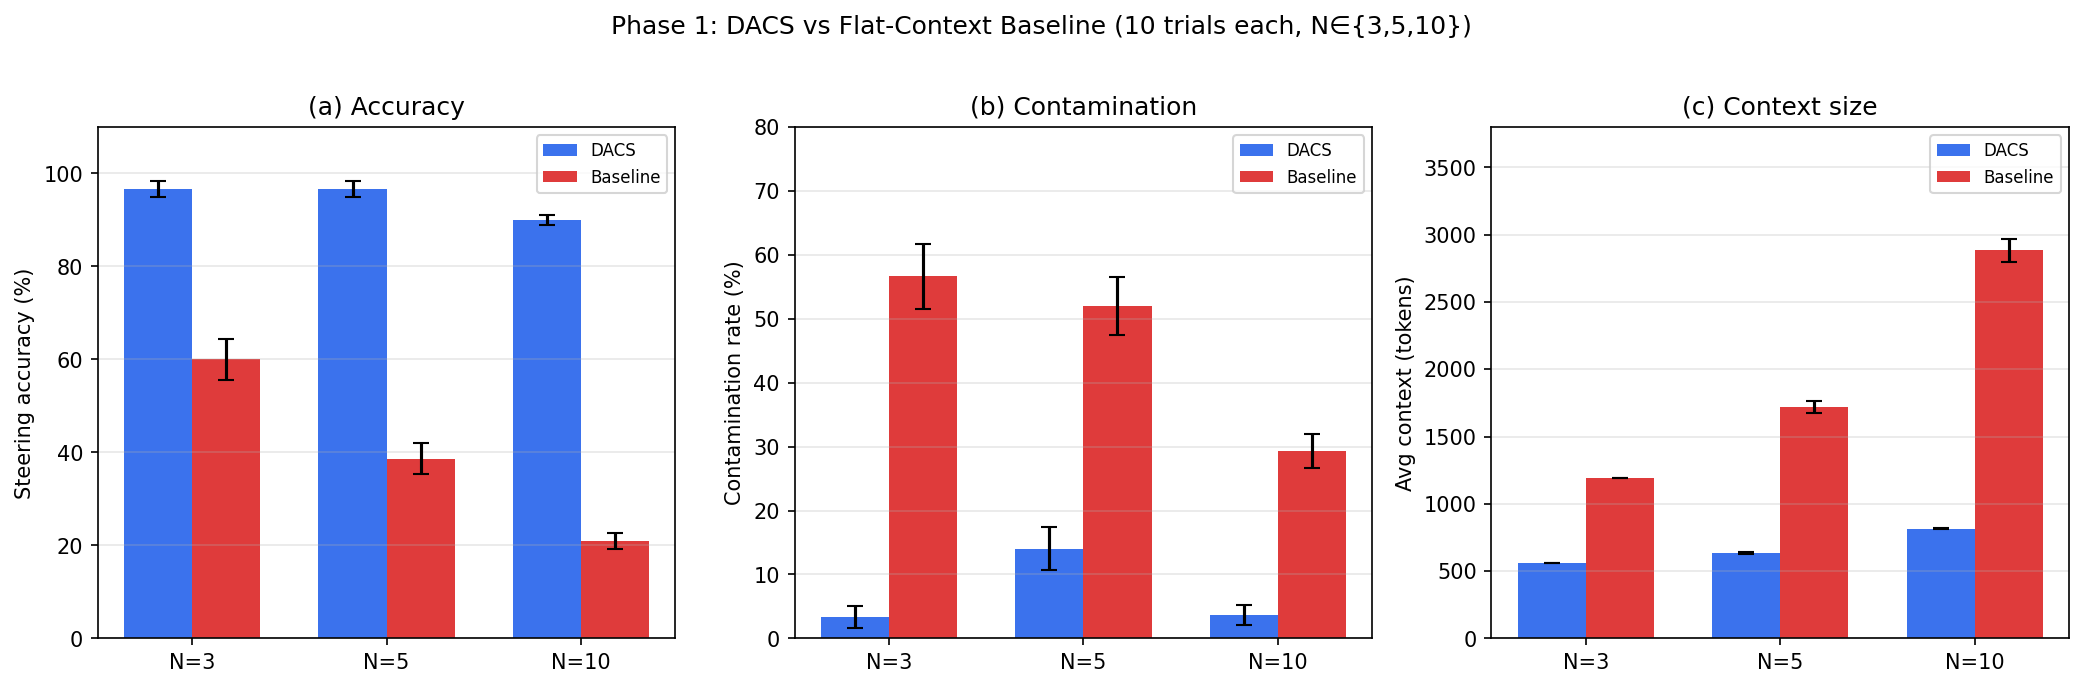
\includegraphics[width=\textwidth]{figures/phase1_overview.png}
  \caption{DACS vs.\ flat-context baseline across $N \in \{3,5,10\}$
  (Phase~1).
  Error bars: $\pm 1$ SE (10 trials each).
  (a) Steering accuracy.
  (b) Wrong-agent contamination.
  (c) Average context tokens at steering time.}
  \label{fig:phase1}
\end{figure}

\subsection{Phase 2: Agent Diversity}

\begin{table}[t]
\caption{Phase~2 results across homogeneous, crossfire, and cascade
scenarios.
Each cell: mean $\pm$ SE over 10 trials.}
\label{tab:phase2}
\centering
\small
\begin{tabular}{llrrrrr}
\toprule
Scenario & Cond. & Accuracy & Contamination & Ctx (tok) & $\Delta$ acc & Ctx ratio \\
\midrule
\multirow{2}{*}{s4 homogeneous ($N=3$)}
  & DACS     & $90.2\pm3.5\%$ & $0.8\pm0.7\%$  & $815\pm10$  & \multirow{2}{*}{$+37.7$pp} & \multirow{2}{*}{$2.29\times$} \\
  & Baseline & $52.5\pm1.7\%$ & $44.2\pm3.1\%$ & $1{,}869\pm49$ & & \\[4pt]
\multirow{2}{*}{s5 crossfire ($N=5$)}
  & DACS     & $96.0\pm0.9\%$ & $0.0\pm0.0\%$ & $911\pm6$   & \multirow{2}{*}{$+59.0$pp} & \multirow{2}{*}{$2.90\times$} \\
  & Baseline & $37.0\pm1.8\%$ & $53.0\pm2.8\%$ & $2{,}643\pm33$ & & \\[4pt]
\multirow{2}{*}{s6 cascade ($N=5$, adversarial)}
  & DACS     & $94.0\pm1.5\%$ & $7.3\pm2.2\%$  & $705\pm10$  & \multirow{2}{*}{$+37.3$pp} & \multirow{2}{*}{$2.65\times$} \\
  & Baseline & $56.7\pm3.2\%$ & $28.7\pm3.4\%$ & $1{,}870\pm38$ & & \\
\bottomrule
\end{tabular}
\end{table}

Table~\ref{tab:phase2} answers RQ3 (does the advantage generalise
across agent heterogeneity?): DACS wins in all three cases by large
margins ($p < 0.0001$ throughout).

\paragraph{Homogeneous agents (s4).}
Even when all three agents share the same domain vocabulary (algorithm
coding), DACS achieves $+37.7$ pp accuracy.
Same-domain sharing reduces baseline contamination relative to Phase~1
heterogeneous scenarios (44\% vs.\ 57\%), but the flat context's
inability to focus on the current decision point still causes baseline
accuracy to fall to 52.5\%.

\paragraph{Maximum diversity (s5).}
The crossfire scenario is DACS's best case: five domains with
guaranteed vocabulary disjointness.
DACS achieves 96.0\% accuracy with 0.0\% contamination.
The 59.0 pp gap is the second-largest observed across all experiments.
Notably, 5 of 8 disagreements in the LLM-as-judge validation
(\S\ref{sec:metrics}) arise in the baseline condition of this
scenario: contaminated responses that accidentally contain a keyword
from the correct domain while addressing a different agent's task.
This demonstrates that keyword false positives in the baseline
condition are themselves evidence of the contamination mechanism, and
that reported baseline accuracy is if anything a slight overestimate.

\paragraph{Adversarial cascade (s6).}
The cascade scenario is designed to challenge DACS: agents produce
outputs that downstream agents depend on, so the flat baseline might
benefit from knowing all agents' histories.
DACS wins by $+37.3$ pp despite this. The flat context does not
help the baseline orchestrator—it still conflates agent contexts at
steering time.
DACS contamination in s6 (7.3\%) is elevated relative to other
scenarios: the legitimate cross-agent references in a pipeline
(e.g., ``retrieval service decided on BM25'') cause some controlled
vocabulary bleed. Nevertheless, accuracy is dominant.

Figure~\ref{fig:phase2} visualises all three metrics for the
heterogeneity scenarios and shows that contamination suppression under
DACS remains robust in both homogeneous and maximally diverse settings.

\begin{figure}[t]
  \centering
  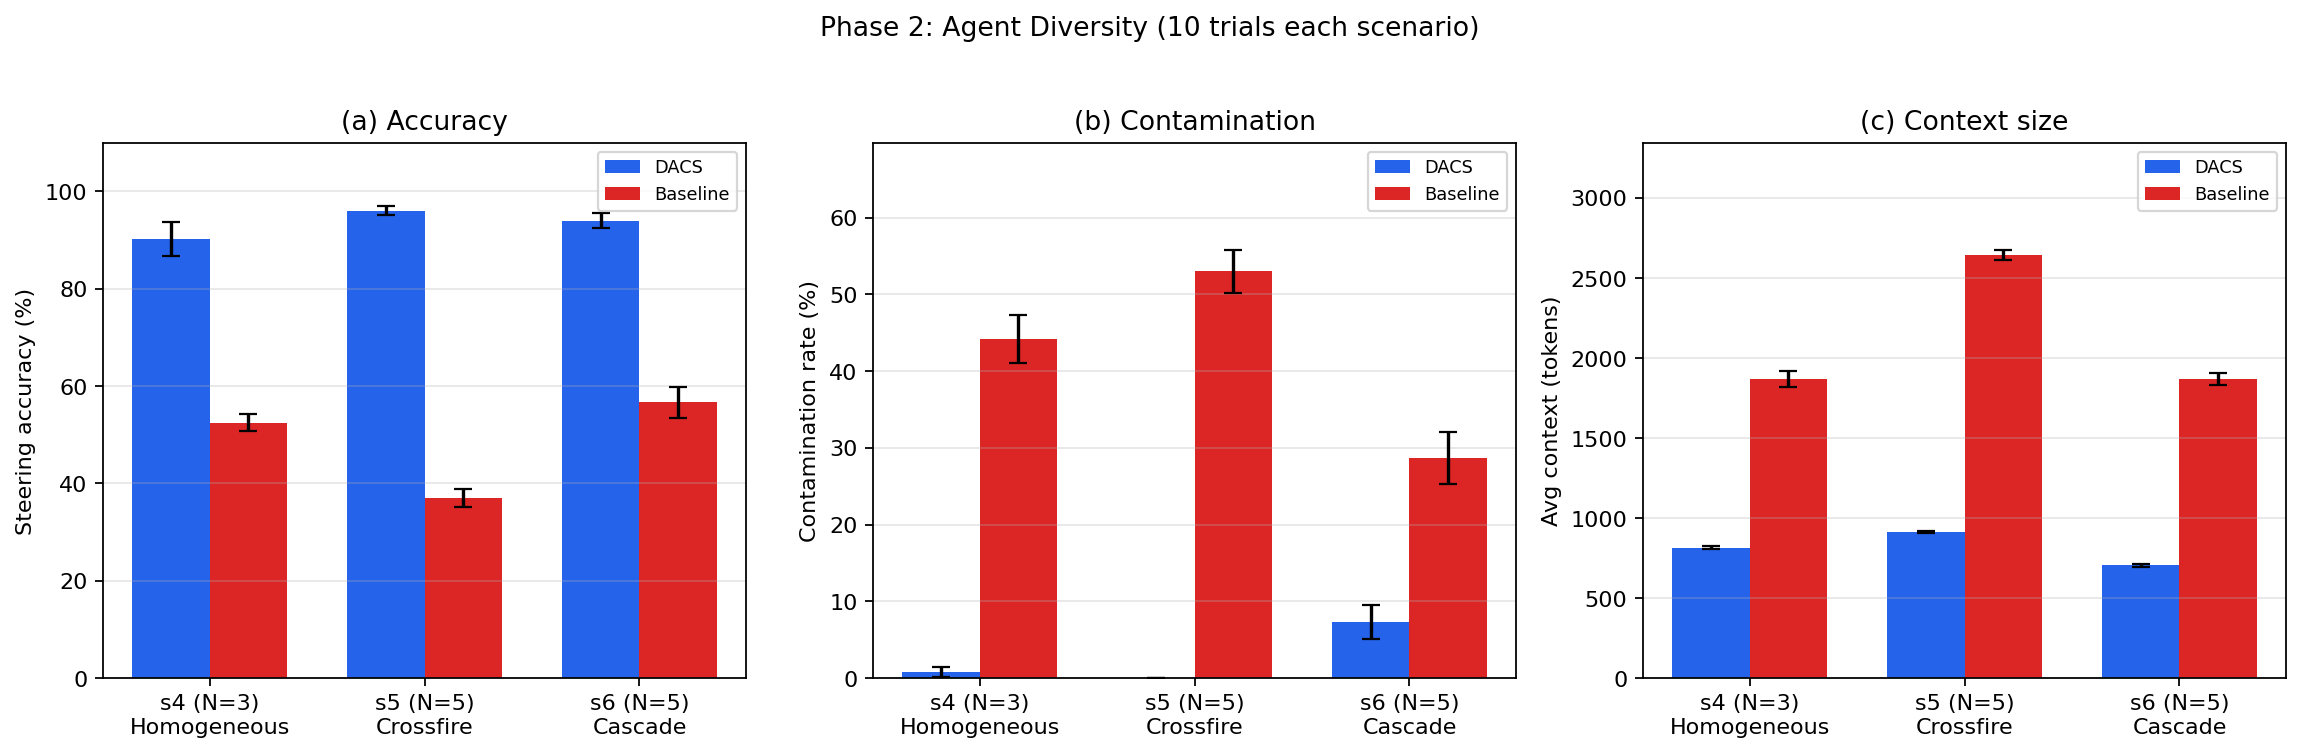
\includegraphics[width=\textwidth]{figures/phase2_overview.png}
  \caption{Phase~2 (agent diversity) results across s4 homogeneous,
  s5 crossfire, and s6 cascade.
  Error bars: $\pm 1$ SE (10 trials each).
  (a) Steering accuracy.
  (b) Wrong-agent contamination.
  (c) Average context tokens at steering time.}
  \label{fig:phase2}
\end{figure}

\subsection{Phase 3: Decision Density Scaling}

\begin{table}[t]
\caption{Phase~3 results: high-density decision scenarios.
$D$ = decisions per agent per trial.
Values are mean $\pm$ SE over 10 trials.}
\label{tab:phase3}
\centering
\small
\begin{tabular}{llrrrrr}
\toprule
Scenario & Cond. & Accuracy & Contamination & Ctx (tok) & $\Delta$ acc & Ctx ratio \\
\midrule
\multirow{2}{*}{s7 ($N=5,\; D=8$)}
  & DACS     & $94.0\pm0.8\%$ & $0.2\pm0.2\%$  & $1{,}654\pm20$ & \multirow{2}{*}{$+59.2$pp} & \multirow{2}{*}{$3.24\times$} \\
  & Baseline & $34.8\pm1.8\%$ & $49.8\pm3.3\%$ & $5{,}364\pm98$  & & \\[4pt]
\multirow{2}{*}{s8 ($N=3,\; D=15$)}
  & DACS     & $98.4\pm0.5\%$ & $0.9\pm0.9\%$  & $2{,}755\pm29$ & \multirow{2}{*}{$+54.2$pp} & \multirow{2}{*}{$2.39\times$} \\
  & Baseline & $44.2\pm1.3\%$ & $51.6\pm2.4\%$ & $6{,}573\pm153$ & & \\
\bottomrule
\end{tabular}
\end{table}

Table~\ref{tab:phase3} answers RQ4 (does the advantage scale with
decision density?): yes. Both scenarios show large, highly significant
gains ($t=30.24$, $p=2 \times 10^{-13}$ for s7; $t=40.30$,
$p=10^{-13}$ for s8).

Figure~\ref{fig:phase3} shows that high decision density increases
baseline context burden sharply while DACS remains comparatively stable,
preserving both accuracy and contamination control.

\begin{figure}[t]
  \centering
  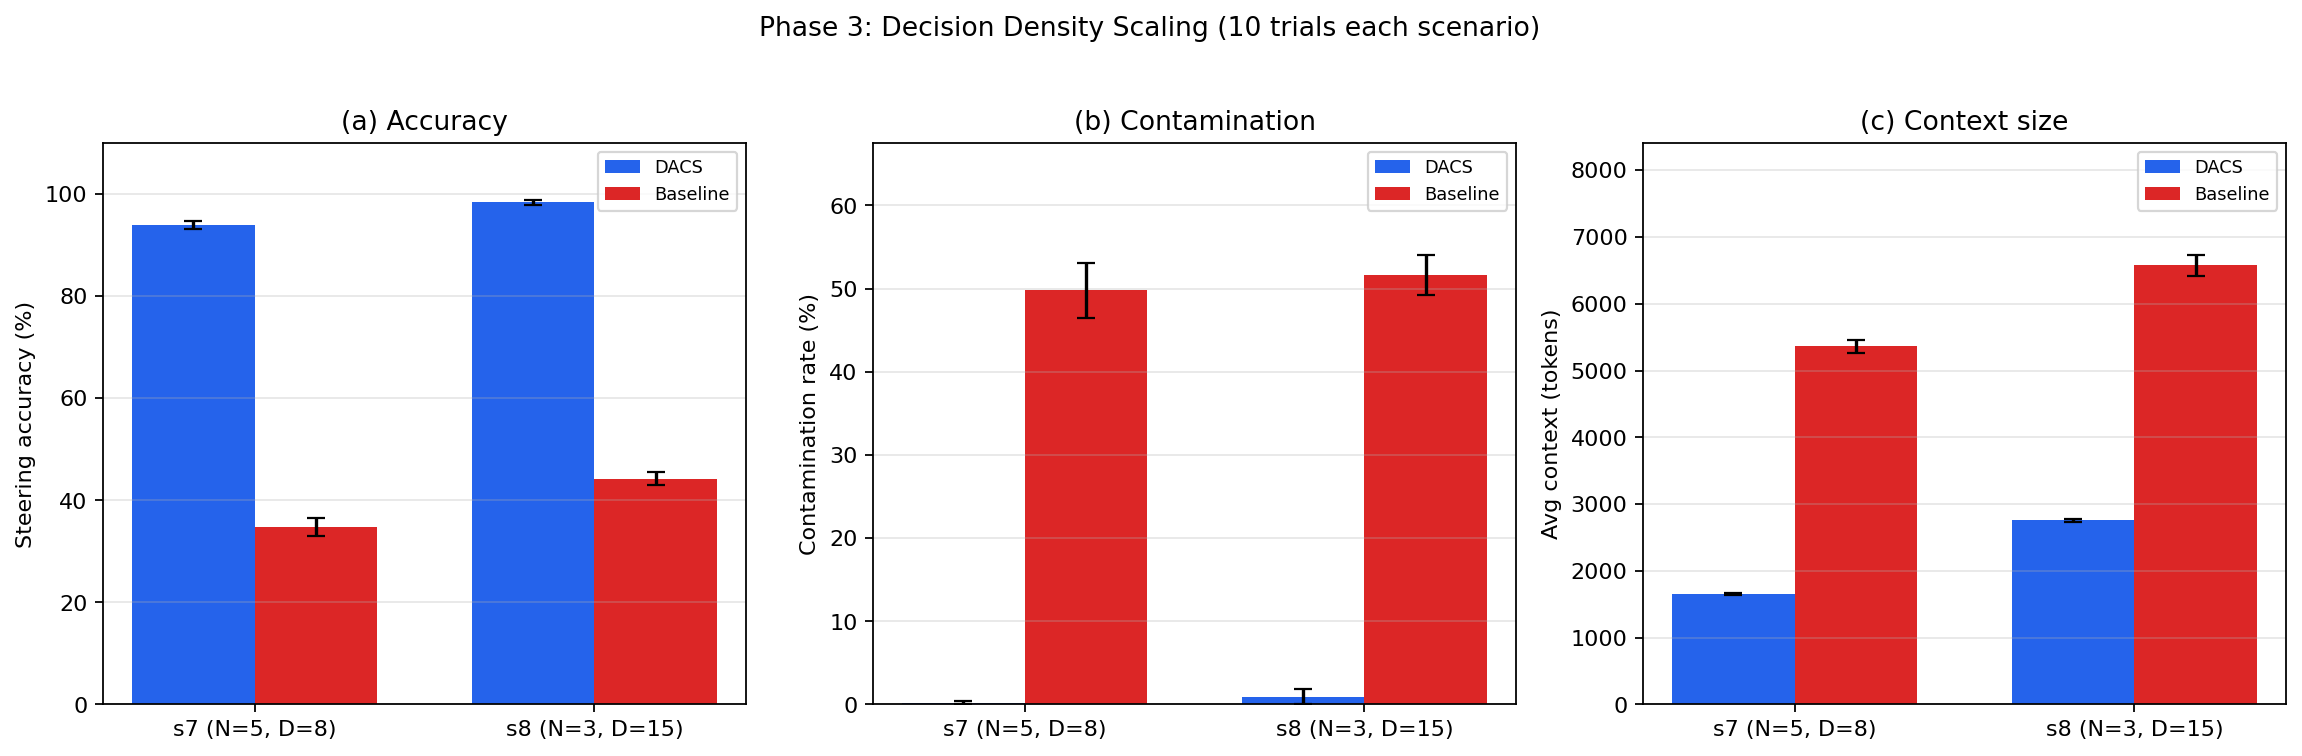
\includegraphics[width=\textwidth]{figures/phase3_overview.png}
  \caption{Phase~3 (decision density scaling) results for s7 ($N=5,
  D=8$) and s8 ($N=3, D=15$).
  Error bars: $\pm 1$ SE (10 trials each).
  (a) Steering accuracy.
  (b) Wrong-agent contamination.
  (c) Average context tokens at steering time.}
  \label{fig:phase3}
\end{figure}

\paragraph{RQ4: Decision density amplifies the baseline's degradation.}
Table~\ref{tab:density} tracks the N=3 and N=5 trajectories across all
three phases as $D$ increases.

\begin{table}[h]
\caption{DACS advantage as a function of decisions per agent $D$,
holding $N$ fixed. Accuracy delta and context efficiency ratio grow
as $D$ increases for the baseline; DACS accuracy is stable.}
\label{tab:density}
\centering
\small
\begin{tabular}{lllrrrrr}
\toprule
Phase & Scenario & $N$ & $D$ & DACS acc & Baseline acc & $\Delta$ & Ctx ratio \\
\midrule
1 & s1\_n3           & 3 & $\approx 3$ & 96.7\% & 60.0\% & $+36.7$pp & $2.12\times$ \\
2 & s4\_n3\_homog.   & 3 & 4           & 90.2\% & 52.5\% & $+37.7$pp & $2.29\times$ \\
3 & s8\_n3\_dense\_d3 & 3 & \textbf{15} & \textbf{98.4\%} & \textbf{44.2\%} & $\mathbf{+54.2}$\textbf{pp} & $2.39\times$ \\
\midrule
1 & s2\_n5           & 5 & $\approx 3$ & 96.7\% & 38.7\% & $+58.0$pp & $2.72\times$ \\
2 & s5\_n5\_crossfire & 5 & 4           & 96.0\% & 37.0\% & $+59.0$pp & $2.90\times$ \\
3 & s7\_n5\_dense\_d2 & 5 & \textbf{8}  & \textbf{94.0\%} & \textbf{34.8\%} & $+59.2$pp & $\mathbf{3.24\times}$ \\
\bottomrule
\end{tabular}
\end{table}

At $N=3$, pushing $D$ from 3 to 15 drops baseline accuracy from 60.0\%
to 44.2\%---a 15.8 pp decline---while DACS accuracy rises slightly
(96.7\% $\to$ 98.4\%).
The accuracy delta jumps from $+36.7$ pp to $+54.2$ pp, a 17.5 pp
increase attributable entirely to decision history depth.
At $N=5$, baseline accuracy falls moderately (38.7\% $\to$ 34.8\% as
$D$ doubles), while DACS stays near 94--96\%.
The context efficiency ratio reaches $3.24\times$ for s7---the highest
recorded for $N=5$---confirming that flat-context token costs grow with
accumulated steering history while DACS costs only reflect the current
agent's history.

DACS's accuracy improvement with depth (98.4\% at $D=15$ vs.\ 96.7\%
at $D=3$) is consistent with the mechanism design: at high $D$, the
focus context contains a richer per-agent history, giving the
orchestrator more signal to make accurate steering decisions.
The flat baseline cannot exploit this signal---it is buried under all
other agents' equally long histories.

\subsection{Cumulative View}

\begin{table}[t]
\caption{All 8 scenarios across three phases.
DACS accuracy is consistently high (90.0--98.4\%); baseline collapses
under agent count and decision density pressure.}
\label{tab:all}
\centering
\small
\begin{tabular}{llllrrr}
\toprule
Phase & Scenario & $N$ & $D$ & DACS & Baseline & $\Delta$ \\
\midrule
1 & s1\_n3                & 3  & $\approx$3 & 96.7\% & 60.0\% & $+36.7$pp \\
1 & s2\_n5                & 5  & $\approx$3 & 96.7\% & 38.7\% & $+58.0$pp \\
1 & s3\_n10               & 10 & $\approx$3 & 90.0\% & 21.0\% & $+69.0$pp \\
2 & s4\_n3\_homogeneous   & 3  & 4          & 90.2\% & 52.5\% & $+37.7$pp \\
2 & s5\_n5\_crossfire     & 5  & 4          & 96.0\% & 37.0\% & $+59.0$pp \\
2 & s6\_n5\_cascade       & 5  & 3          & 94.0\% & 56.7\% & $+37.3$pp \\
3 & s7\_n5\_dense\_d2     & 5  & 8          & 94.0\% & 34.8\% & $+59.2$pp \\
3 & s8\_n3\_dense\_d3     & 3  & 15         & 98.4\% & 44.2\% & $+54.2$pp \\
\bottomrule
\end{tabular}
\end{table}

Across all 8 scenarios and 160 trials (Table~\ref{tab:all}), DACS
accuracy ranges $90.0$--$98.4\%$.
The minimum DACS advantage is $+36.7$ pp; the maximum is $+69.0$ pp.
DACS has never lost to the flat-context baseline in any scenario.
The results answer all four research questions:
\textbf{RQ1}~(Does DACS outperform the baseline?): yes, in all 8
scenarios at $p<0.0001$.
\textbf{RQ2}~(Does the advantage grow with $N$?): yes, from
$+36.7$ pp at $N=3$ to $+69.0$ pp at $N=10$.
\textbf{RQ3}~(Does the advantage hold across agent heterogeneity?):
yes, including the adversarial cascade scenario.
\textbf{RQ4}~(Does decision density amplify the advantage?): yes,
$+17.5$ pp increase in the delta as $D$ quintuples at $N=3$.

%-----------------------------------------------------------------------
\section{Discussion}
\label{sec:discussion}

\subsection{Why DACS Works}

The mechanism's effectiveness follows directly from what it removes from
the context window.
In the flat baseline, when $a_i$ asks ``should I use recursive or
iterative traversal for my BST inorder walk?'', the context simultaneously
holds a research agent's detailed transformer attention analysis and a
data processor's CSV encoding problem, containing domain keywords
(``attention'', ``heads'', ``encoding'', ``UTF-8'') that have nothing to
do with the correct answer.
The LLM anchors its response to whichever content pattern captures its
attention—an effect we measure as both inaccuracy and contamination.

DACS removes this anchor competition entirely.
In \textsc{Focus}$(a_i)$ mode, the context contains $a_i$'s task
description and steering history plus compact status lines for other
agents (``a2: RUNNING, transformer survey, 3/5 steps done'').
The correct-answer vocabulary dominates the context by construction.

\subsection{Why High Decision Density Hurts the Baseline}

Phase~3 reveals a compounding mechanism.
As $D$ grows, the flat context accumulates not just $N$ agents'
\emph{current} states but their full steering \emph{histories}.
At $D=15$, a 3-agent flat context holds 45 steering interaction pairs,
each injecting domain vocabulary that drowns out the signal for the
current decision.
DACS's focus context at $D=15$ holds only $a_i$'s 15-interaction
history---precisely the relevant signal---plus three compact registry
lines for the other agents.
The result is that DACS accuracy at $D=15$ (98.4\%) \emph{exceeds} its
accuracy at $D\approx 3$ (96.7\%): more history in the focus
context is additive signal, not noise.

\subsection{Relation to Hierarchical Routing}

DACS is orthogonal to hierarchical agent architectures
(AgentOrchestra~\citep{agentorchestra2025},
AdaptOrch~\citep{adaptorch2025b}).
Hierarchical routing reduces how many agent threads reach the
orchestrator at all.
DACS controls what the orchestrator holds in its context at each
steering moment during execution.
A production system could combine both: hierarchical routing limits the
active agent pool, and DACS ensures that within that pool, each steering
interaction is isolated.

\subsection{Limitations}

\paragraph{Benchmark scope.}
The task suite uses keyword matching to evaluate steering accuracy.
This is conservative (multi-word phrases and paraphrases are not captured)
and may produce false-positive contamination detections when domains share
vocabulary.
LLM-as-judge validation across all three phases confirms metric validity:
Phase~2 $\kappa=0.956$; Phase~3 s8 $\kappa=0.886$; Phase~3 s7
$\kappa=0.933$ (mean $\kappa=0.909$, all well above the $\kappa{\geq}0.80$
``substantial agreement'' threshold).

\paragraph{Synthetic agents.}
Our agent stubs simulate decision points with pre-defined timing and
question templates.
Real agents have irregular steering request patterns, potentially large
partial outputs, and multi-turn steering histories.
Phase~3 partially addresses this by extending decision histories to $D=15$;
however, real-world $D$ values could be much higher.

\paragraph{Single model and context budget.}
All experiments use MiniMax-M2.7 at a 204{,}800-token budget.
With a smaller budget, context pollution effects would be more severe.
Results may differ across model families with different attention
characteristics.

\paragraph{Interrupt handling not experimentally isolated.}
The interrupt protocol (transition~\eqref{eq:t3}) was exercised naturally in
experiments but not ablated independently.

\subsection{Future Work}

\begin{itemize}
  \item \textbf{LLM-as-judge for Phase~3.} Full judge validation on
  s8\_n3\_dense\_d3 (900 decisions) to confirm Phase~3 keyword scores.
  \item \textbf{User responsiveness.} Measure latency from user message
  to orchestrator response under DACS vs.\ baseline at varying $N$ and
  queue depth.
  \item \textbf{Real application integration.} Integrate DACS as a
  drop-in context management layer in an existing production multi-agent
  system.
  \item \textbf{Very high $D$.} Extend Phase~3 to $D \in \{30, 50, 100\}$
  to probe where, if anywhere, DACS accuracy degrades as per-agent
  history grows very large.
\end{itemize}

%-----------------------------------------------------------------------
\section{Conclusion}
\label{sec:conclusion}

We presented DACS, a dynamic attentional context scoping mechanism that
solves context pollution in multi-agent LLM orchestration through
agent-triggered asymmetric focus sessions.
The mechanism is exact (not approximate), sub-linear in agent count, and
compatible with existing orchestration architectures.

Across 160 experimental trials in 8 scenarios spanning three phases,
DACS achieves $90.0$--$98.4\%$ steering accuracy versus $21.0$--$60.0\%$
for the flat-context baseline, reduces wrong-agent contamination from
$28$--$57\%$ to $0$--$9\%$, and exhibits growing context efficiency
(2.12--3.53$\times$) as $N$ increases.
The advantage is robust to agent heterogeneity (Phase~2), holds even in
pipeline-dependent adversarial scenarios, and \emph{compounds with
decision density} (Phase~3): quintupling $D$ from 3 to 15 causes baseline
accuracy to fall by 15.8 pp while DACS accuracy is unchanged or improves.

The core contribution is demonstrating that \emph{what is in the
orchestrator's context window at the moment of steering} is the
dominant variable for multi-agent steering accuracy---not model size,
not topology, not memory compression---and that a simple, deterministic
mode-switch mechanism suffices to control it effectively across a
wide range of agent counts, diversity structures, and decision densities.

%-----------------------------------------------------------------------
\bibliographystyle{plainnat}
\bibliography{refs}

\end{document}
